\section{Linux Power Governors}\label{sec:linux-powergov}

\begin{figure}[h]
  \begin{center}
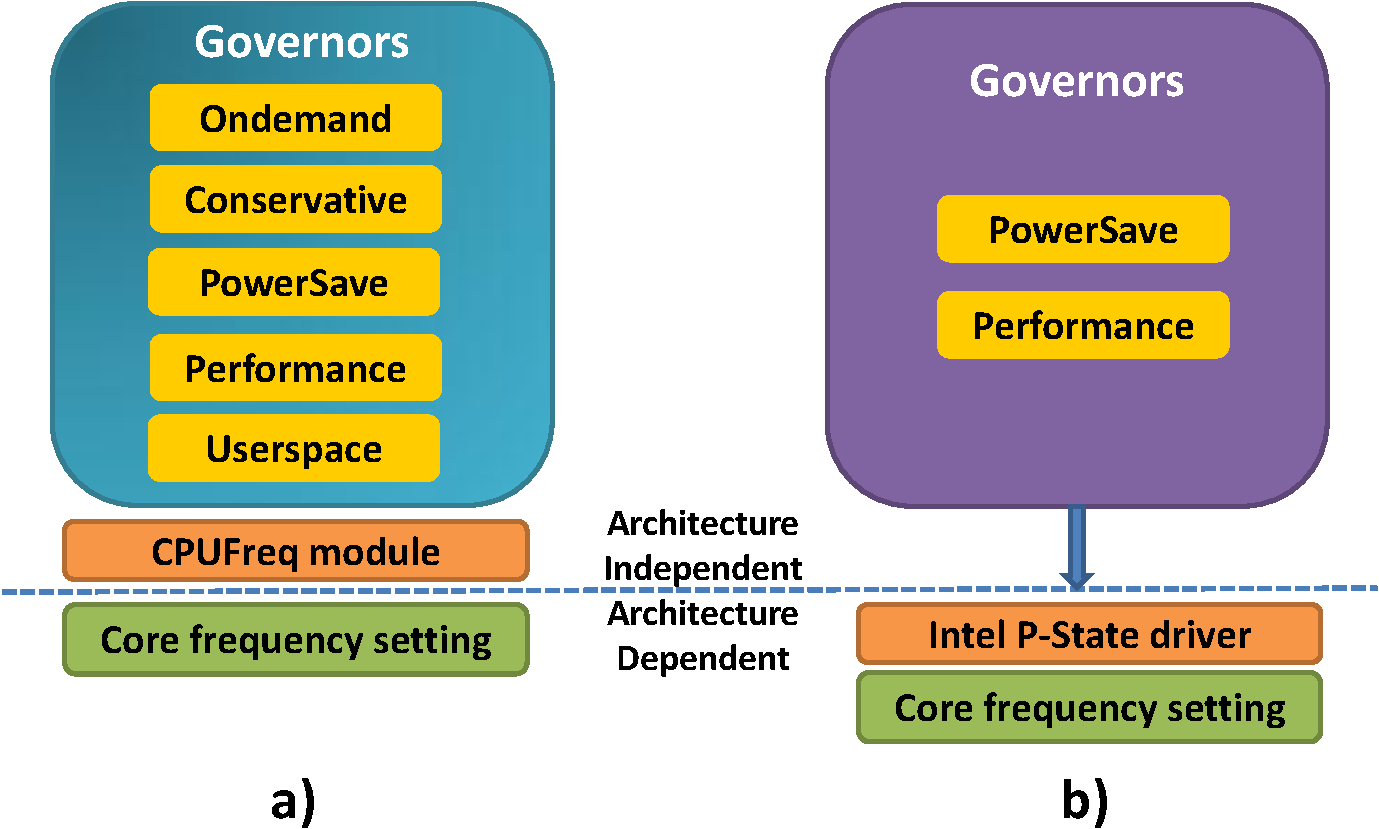
\includegraphics[width=\linewidth]{figs/gov-crop.pdf}
  \end{center}
  \vspace{-0.1in}
  \caption{Freq reduced by 30\%}
	\label{fig:gov}
\end{figure}



CPU frequency scaling enables the operating system to scale the CPU frequency up or down in order to save power. CPU frequencies can be scaled automatically depending on the system load, in response to ACPI events, or manually by user space programs. The infrastructure available in Linux kernel to perform frequency scaling is called \emph{cpufreq}. Most cpufreq drivers or even most cpu frequency scaling algorithms only offer the CPU to be set to one frequency. In order to offer dynamic frequency scaling, the cpufreq governor must be able to tell these drivers of a "target frequency". Similar to \emph{cpufreq}, recently linux power governors can be monitored using \emph{cpumonitor} utility which gives the running frequency information as well as performance statistics under that governor.

There are various power governors available in Linux. Some of the most popular ones are listed below:
\subsection{Performance}
This governor sets the CPU statically to a maximum frequency. This governor comes in handy in today’s phones, which implement a faster race to idle. Race-to-idle is the process by which a phone completes a given task, such as syncing email, and returns the CPU to the extremely efficient low-power state. This governor however, relies on a kernel that properly implements low power CPU C states.

\subsection{Powersave}
This governor is the opposite of Performance governor and sets the CPU statically to the lowest frequency set by the user.

\subsection{Userspace}
This governor allows the user or any user space program running with UID “root” to set the CPU to a specific frequency. This governor is more common amongst server and desktop PCs and is seldom used in mobile devices.

\subsection{On Demand}
This governor sets the CPU frequency depending on the current usage. To do this the CPU must have the capability to switch between frequencies very quickly. In general, this governor tries to run the CPU load at high frequency. If the CPU load placed by the user abates, the Ondemand governor will slowly step back down through the kernel's frequency steppings until it settles at the lowest possible frequency, or the user executes another task to demand a ramp.
Ondemand scales its frequency in a work queue context. In other words, once the task that triggered the frequency ramp is finished, OnDemand will attempt to move the frequency back to minimum. If the user executes another task that triggers OnDemand's ramp, the frequency will bounce from minimum to maximum.
This governor provides tunable parameters like sampling rate, the rate at which governor takes a look at CPU usage and makes a decision about frequency and sampling down factor, the rate at which the governor makes a decision on when to decrease the frequency while running at top speed

\subsection{Conservative}
This governor much like the ondemand governor, sets the CPU depending on the current usage.  It differs in behaviour in that it gracefully increases and decreases the CPU speed rather than jumping to maximum speed the moment there is any load on the CPU. This behaviour is more suitable in a battery powered environment.
This governor provides tunable parameters like frequency steps, which describes what percentage steps the cpu freq should be increased and decreased smoothly by.

\subsection{Min- Max}
This governor as the name suggests only makes use of minimum and maximum frequencies depending upon the CPU load and does not use any intermediate frequencies.

\subsection{Interactive}
Much like the OnDemand governor, the Interactive governor dynamically scales CPU frequency in response to the workload placed on the CPU by the user. However, this governor is significantly more responsive than OnDemand, because it's faster at scaling to maximum frequency.
Unlike Ondemand governor, which scales clockspeed in the context of a work queue, Interactive governor scales the clockspeed over the course of a timer set arbitrarily by the kernel. In other words, if an application demands a ramp to maximum frequency by placing 100\% load on the CPU, an user can execute another task before the governor starts reducing CPU frequency. The timer also renders this governor better suitable to utilize intermediate frequencies.

\fixme{Need to include the Intel P-State Drivers information here}
